\documentclass{beamer}
% \usetheme{Copenhagen}
% \usepackage{minted}
\usepackage{listings}
\usepackage{bm}
\usepackage{amsmath}
\usepackage{sagetex}
\usepackage{float}
\usepackage{subfig}

\usepackage[
    % style=alphabetic,
    style=numeric,
    maxbibnames=99,
    maxnames=99
]{biblatex} %Imports biblatex package
\addbibresource{../bibliography.bib}

% \setbeamertemplate{bibliography item}{\insertbiblabel}

\definecolor{codegreen}{rgb}{0,0.6,0}
\definecolor{codegray}{rgb}{0.5,0.5,0.5}
\definecolor{codepurple}{rgb}{0.58,0,0.82}
\definecolor{backcolour}{rgb}{0.95,0.95,0.92}

\lstdefinestyle{mystyle}{
    backgroundcolor=\color{backcolour},   
    commentstyle=\color{codegreen},
    keywordstyle=\color{magenta},
    numberstyle=\tiny\color{codegray},
    stringstyle=\color{codepurple},
    basicstyle=\ttfamily\footnotesize,
    breakatwhitespace=false,         
    breaklines=true,                 
    captionpos=b,                    
    keepspaces=true,                 
    numbers=left,                    
    numbersep=5pt,                  
    showspaces=false,                
    showstringspaces=false,
    showtabs=false,                  
    tabsize=2
}

\lstset{style=mystyle}


% \setcounter{tocdepth}{1}

\AtBeginSection{%
    \begin{frame}
         \frametitle{Outline}
        \tableofcontents[currentsection, hideallsubsections]
    \end{frame}
    \begin{frame}
        \tableofcontents[sections=\value{section}]
    \end{frame}
}

\newcommand\Wider[2][3em]{%
\makebox[\linewidth][c]{%
    \begin{minipage}{\dimexpr\textwidth+#1\relax}
        \raggedright#2
    \end{minipage}%
}%
}

\title{Implementation of a library for convolutional neural networks in futhark}
% \subtitle{Using Beamer}
\author{Alexander Nortung}
\institute{University of Copenhagen}
\date{2022-06-21}

\begin{document}

\begin{frame}
    \titlepage
\end{frame}

% \begin{frame}
%     \frametitle{Outline}
%     \tableofcontents[hideallsubsections]
% \end{frame}

\section{Background}

\subsection{Futhark}

\begin{frame}
    \frametitle{Futhark}
    \begin{itemize}
        \item Functional programming language
        \item Effecient
        \item GPU code
    \end{itemize}
\end{frame}

\begin{frame}[fragile]
    \frametitle{A simple example}
    % \begin{minted}{futhark}
    %     def main (x: i64) : i64 =
    %         let a
    % \end{minted}
    Consider this program
    \begin{lstlisting}
def main (x: i64) : i64 =
    let a = 12
    in a + x
    \end{lstlisting}
    \pause
    \begin{description}
        \item[def] Defines a function
        \item[(x: i64)] A parameter named \texttt{x} with type of \texttt{i64}
        \item[: i64] returns a type is i64
        \pause
        \item[let] Creates a new variable
        \item[in] What should be reutrned (only needed with let)
    \end{description}
    \pause
    The main function is executed by default
\end{frame}

\begin{frame}[fragile]
    \frametitle{Modules}
    Being able to isolate code and functions is essential for building libraries and larger applications.
    \begin{lstlisting}
-- a.fut
module a = {
    def sub 't (a: t) (b: t) : t =
        a - b
}
    \end{lstlisting}
    \pause
    We can use the module in a program
    \begin{lstlisting}
-- program.fut
import "a"
def main =
    a.sub 6 7
    \end{lstlisting}
\end{frame}

\begin{frame}[fragile]
    \frametitle{Polymorphism}
    We saw in the previous slide that we could use a type \texttt{'t} which is a polymortphic type
    \begin{lstlisting}
def sub 't (a: t) (b: t) : t =
    a - b
    \end{lstlisting}
    \pause
    examples:
    \begin{lstlisting}
sub 10.0f32 0.5f32
sub 10u8 1u8
    \end{lstlisting}
\end{frame}

\begin{frame}[fragile]
    \frametitle{Size types}
    An important part of Futhark is its use of size types
    \begin{lstlisting}
def sub_array 't (a: [10]t) (b: [10]t) : [10]t =
    map2 (-) a b
    \end{lstlisting}
    \pause
    Named or dynamic size types gives more flexibility
    \begin{lstlisting}
def sub_array 't [sz] (a: [sz]t) (b: [sz]t) : [sz]t =
    map2 (-) a b
    \end{lstlisting}
    \pause
    This would work too, since we do not use the size anywhere.
    \begin{lstlisting}
def sub_array 't (a: []t) (b: []t) : []t =
    map2 (-) a b
    \end{lstlisting}
\end{frame}

\begin{frame}[fragile]
    \frametitle{Tuples and records}
    Tuples can hold different types of values, like other languages

    An example tuple:
    \begin{lstlisting}
let tup = (10i64, 400f64)
    \end{lstlisting}
    \pause
    An example record:
    \begin{lstlisting}
let record = { a: 100, b: 32 }
    \end{lstlisting}
    \pause
    Tuples' and records' values can be accessed with dot notation
    \begin{lstlisting}
tup.0
record.a
    \end{lstlisting}
    \pause
    Or their values can be accessed by destructuring
    \begin{lstlisting}
let (v1, v2) = tup
let { a, b = myB }
    \end{lstlisting}
\end{frame}

\begin{frame}
    \frametitle{Limitations}
    \begin{itemize}
        \item Regular arrays
        \item Arrays cannot contain functions
        \item Size types cannot use arithemetic e.g. \texttt{[a+b-1]}
        \item Parameters cannot come from tuples or records
    \end{itemize}
\end{frame}

\subsection{Gradient descent}

\begin{frame}
    \frametitle{Gradient descent}
    Gradient descent is an iterative process used to find a minima of a function.
    \pause
    By using the derivative of the function we can move a point $\bm{x}$ toward the minima for each iteration.
    $$\bm{x}_{i+1} = \bm{x}_i - \alpha \nabla f(\bm{x})$$
\end{frame}

\begin{frame}[fragile]
    \frametitle{Gradient descent simple example}
    \begin{sageblock}
f(x) = 3 * (x**3) - 25 * (x**2) - 1
fp(x) = derivative(f(x), x)
x1 = 9
a = 0.005
p1 = point((x1, f(x1)), color="red", size=30)
    \end{sageblock}
    \begin{figure}
        \centering
        \sageplot[width=0.5\textwidth]{p1 + plot(f, xmin=-2, xmax=9.50)}
    \end{figure}
    \begin{sageblock}
x2 = x1 - a * fp(x1)
    \end{sageblock}

    % $$x_2 = \sage{x2}$$
\end{frame}

\begin{frame}[fragile]
    \frametitle{Gradient descent simple example}
    \begin{sageblock}
p2 = point((x2, f(x2)), color="red", size=30)
    \end{sageblock}
    \begin{figure}
        \centering
        \sageplot[width=0.5\textwidth]{p2 + plot(f, xmin=-2, xmax=9.50)}
    \end{figure}
    \begin{sageblock}
x3 = x2 - a * fp(x2)
    \end{sageblock}
\end{frame}

\begin{frame}[fragile]
    \frametitle{Gradient descent simple example}
    \begin{sageblock}
p3 = point((x3, f(x3)), color="red", size=30)
    \end{sageblock}
    \begin{figure}
        \centering
        \sageplot[width=0.5\textwidth]{p3 + plot(f, xmin=-2, xmax=9.50)}
    \end{figure}
    $$x_3 = \sage{x3}$$
\end{frame}

\begin{frame}
    \frametitle{Gradient descent}
    For a function with only one parameter the gradient is simply the derivative of the function.

    With multiple parameters it is a vector of each partial derivative
    $$\nabla f(x_1, ..., x_n) = \left( \begin{array}{c}
    \frac{\partial f}{\partial x_1}\\
    \vdots\\
    \frac{\partial f}{\partial x_n}\\
\end{array} \right)$$
\end{frame}


\section{Neural networks}

\begin{frame}
    \frametitle{Neural networks}

    \begin{itemize}
        \item Machine learning model
        \item Layers
        \item Recognize and predict patterns
        \item Propagation
        \item Training
    \end{itemize}

    \begin{figure}
        \centering
        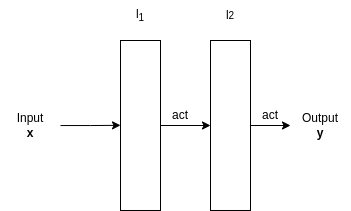
\includegraphics[width=0.5\textwidth]{../assets/nn-simple-example.png}
    \end{figure}
\end{frame}

\subsection{Fully connected layer}

\begin{frame}
    \frametitle{Fully connected layer}

    \begin{itemize}
        \item Used with convolutional layers
        \item Linearly seperable
    \end{itemize}

    \begin{columns}
        \begin{column}{0.5\textwidth}
            Example
            \begin{figure}
                \centering
                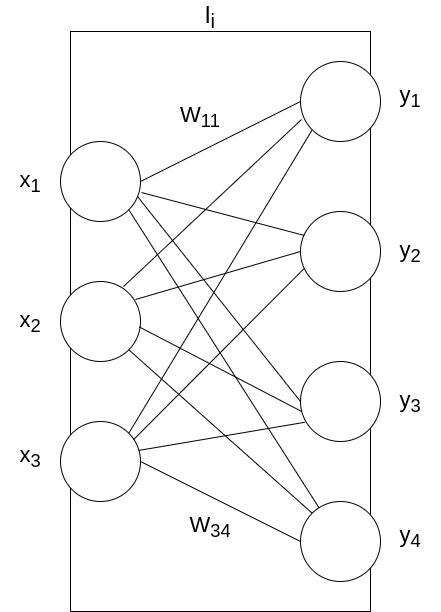
\includegraphics[width=0.6\textwidth]{../assets/linear-layer-example.png}
            \end{figure}
        \end{column}
        \pause
        \begin{column}{0.5\textwidth}
            General
            \begin{figure}
                \centering
                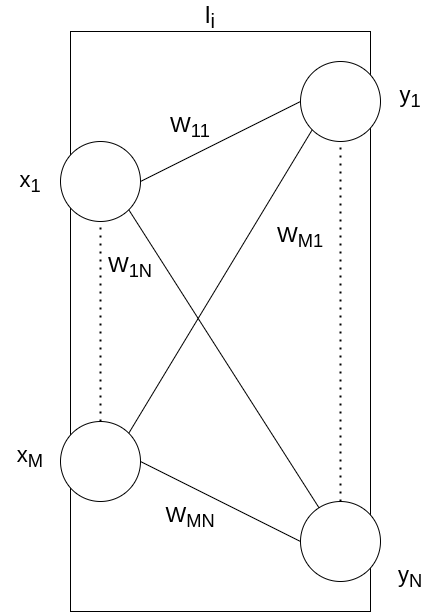
\includegraphics[width=0.6\textwidth]{../assets/linear-layer.png}
            \end{figure}
        \end{column}
    \end{columns}
\end{frame}

\begin{frame}
    \frametitle{Fully connected layer forward propagation}
    The value from each input $x_i$ is multiplied with a weight $w_{ij}$ and summed together in output $y_j$.
    \begin{itemize}
        \item Bias
    \end{itemize}

    \begin{figure}
        \centering
        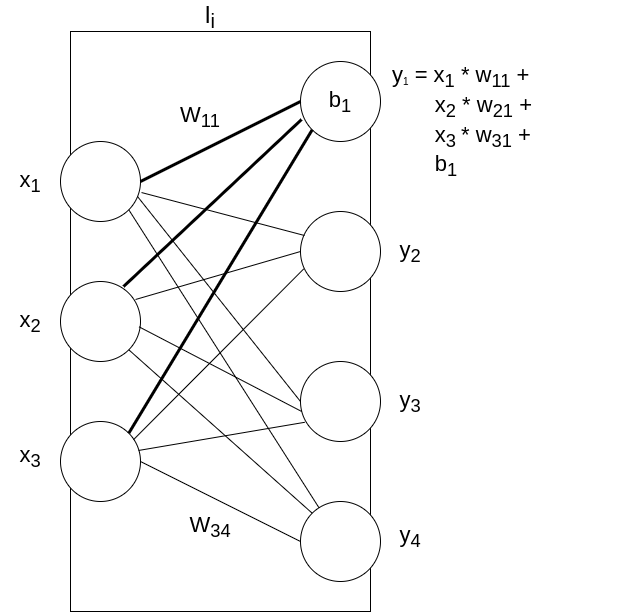
\includegraphics[width=0.5\textwidth]{../assets/linear-layer-linear-propagation.drawio.png}
    \end{figure}
\end{frame}

\begin{frame}
    \frametitle{Fully connected layer forward propagation}

    The forward propagation can be expressed as the following
    $$y_j = b_j + \sum^M_{i=1} w_{ji}x_i$$
    Where $j = 1...M$

    \pause
    And as an expression for all outputs
    $$\bm{y} = \bm{b} + \bm{Wx}$$
\end{frame}

\subsection{Activation functions}

\begin{frame}
    \frametitle{Activation Functions}
    Activation functions are applied to each value after a layer
    \begin{itemize}
        \item Non-linearity
        \item Better fitting
    \end{itemize}
    \pause

    \begin{table}[H]
    \centering
    \begin{tabular}{|c|c|}\hline
    \textbf{Function} & $\bm{\sigma}$ \\\hline
    tanh     & $\frac{e^x - e^{-y}}{e^x + e^{-y}}$ \\\hline
    ReLU     & $max(0, y)$ \\\hline
    sigmoid  & $\frac{1}{1+e^{-y}}$ \\\hline
    softmax  & $\frac{e^{y'}}{\sum^K_{k=1} e^{y_k}}$ \\\hline
    \end{tabular}
    \caption{A list of common activation functions.}
    \label{tab:activation}
    \end{table}
\end{frame}

\subsection{Convolutional layer}

\begin{frame}
    \frametitle{Convolutional layer}
    The convolutional layer is used to extract features from a structured data such as images.
    \begin{itemize}
        \item More layers $\rightarrow$ more features
    \end{itemize}
\end{frame}

\begin{frame}
    \frametitle{Convolutional layer}
    \begin{itemize}
        \item Input
        \item Channels
        \item Kernel
        \item Feature maps
    \end{itemize}
    \pause
    Consider the following input data and kernel

    \begin{figure}
        \centering
        \hfill
        \subfloat[][An example for a $3 \times 3$ input to a convolutional layer]{$\begin{bmatrix}
            X_{11} & X_{12} & X_{13} \\
            X_{21} & X_{22} & X_{23} \\
            X_{31} & X_{32} & X_{33} 
        \end{bmatrix}$}
        \hfill
        \subfloat[][An example for a $2\times 2$ kernel]{$\begin{bmatrix}
            K_{11} & K_{12} \\
            K_{21} & K_{22}
        \end{bmatrix}$}
        \hfill
        \null
        \caption{An example for an input and a kernel to be used in a convolutional layer}
        \label{fig:conv_input_and_kernel}
    \end{figure}
\end{frame}

\begin{frame}
    \frametitle{Convolutional layer example}

    \begin{figure}
        \centering
        $$\begin{bmatrix}
            \color{red} X_{11} & \color{red} X_{12} & X_{13} \\
            \color{red} X_{21} & \color{red} X_{22} & X_{23} \\
            X_{31} & X_{32} & X_{33} 
        \end{bmatrix} \otimes K \Rightarrow \begin{bmatrix}
            \color{red} X_{11} K_{11} + X_{12} K_{12} + X_{21} K_{21} + X_{22} K_{22} & \\
             &
        \end{bmatrix}$$\\
        \pause
        $$\begin{bmatrix}
            X_{11} & \color{red} X_{12} & \color{red} X_{13} \\
            X_{21} & \color{red} X_{22} & \color{red} X_{23} \\
            X_{31} & X_{32} & X_{33} 
        \end{bmatrix} \otimes K \Rightarrow \begin{bmatrix}
             Y''_{11} &\color{red} X_{12} K_{12} + X_{13} K_{13} + X_{22} K_{22} + X_{23} K_{23} \\
             &
        \end{bmatrix}$$\\
        \pause
        $$\begin{bmatrix}
            X_{11} & X_{12} & X_{13} \\
            \color{red} X_{21} & \color{red} X_{22} & X_{23} \\
            \color{red} X_{31} & \color{red} X_{32} & X_{33}
        \end{bmatrix} \otimes K \Rightarrow \begin{bmatrix}
            Y''_{11} & Y''_{12} \\
            \color{red} X_{21} K_{21} + X_{22} K_{22} + X_{31} K_{31} + X_{32} K_{32} & 
        \end{bmatrix}$$\\
        \pause
        $$\begin{bmatrix}
            X_{11} & X_{12} & X_{13} \\
            X_{21} & \color{red} X_{22} & \color{red} X_{23} \\
            X_{31} & \color{red} X_{32} & \color{red} X_{33}
        \end{bmatrix} \otimes K \Rightarrow \begin{bmatrix}
             Y''_{11} & Y''_{12} \\
             Y''_{21} & \color{red} X_{22} K_{22} + X_{23} K_{23} + X_{32} K_{32} + X_{33} K_{33}
        \end{bmatrix}$$\\
        \label{fig:conv_operation}
    \end{figure}
\end{frame}

\begin{frame}
    \frametitle{Convolutional layer stride example}
    A stride can also be used to reduce number of operations and downsample.

    \begin{figure}
        \centering
        $$\begin{bmatrix}
            \color{red} X_{11} & \color{red} X_{12} & X_{13} & X_{14} \\
            \color{red} X_{21} & \color{red} X_{22} & X_{23} & X_{24} \\
            X_{31} & X_{32} & X_{33} & X_{34}
        \end{bmatrix} \otimes K \Rightarrow ...$$\\
        $$\begin{bmatrix}
            X_{11} & X_{12} & \color{red} X_{13} & \color{red} X_{14} \\
            X_{21} & X_{22} & \color{red} X_{23} & \color{red} X_{24} \\
            X_{31} & X_{32} & X_{33} & X_{34}
        \end{bmatrix} \otimes K \Rightarrow ...$$\\
        \label{fig:conv_operation_with_stride}
    \end{figure}
\end{frame}

\begin{frame}
    \frametitle{Convolutional layer generalized}
    The outputs can be described as the following expression
    $$Y_{ij} = b + \sum^{C_{in}}_{c = 1} \sum^{i \cdot s_x + k_x}_{i_2 = i \cdot s_x} \sum^{j \cdot s_y + k_y}_{j_2 = j \cdot s_y} X_{ci_2j_2} K_{ci_2j_2} $$
    \pause

    \begin{description}
        \item[$C_{in}$] The number of in channels
        \item[$s_x$ $s_y$] The stride for each dimension
        \item[$k_x$ $k_y$] The size of the kernel
    \end{description}
    \pause

    $$i = 1, ..., \left\lfloor\frac{n_x - k_x}{s_x}\right\rfloor + 1$$
    $$j = 1, ..., \left\lfloor\frac{n_y - k_y}{s_y}\right\rfloor + 1$$

    \begin{description}
        \item[$n_x$ $n_y$] The size of the input
    \end{description}
\end{frame}

\subsection{Maxpooling layer}

\begin{frame}
    \frametitle{Maxpooling layer}

    \begin{itemize}
        \item Downsampling to avoid overfitting
        \item Feature maps
        \pause
        \item Partitioning $\rightarrow$ max
    \end{itemize}


    \begin{figure}[htpb]
        \centering
        $$\begin{bmatrix}
            \color{red}1 & \color{red} 2 & \color{green} 3 & \color{green} 4 \\
            \color{red}8 & \color{red}9 & \color{green}10 & \color{green}11 \\
            \color{blue}7 & \color{blue}1 & \color{magenta}2 & \color{magenta}6 \\
            \color{blue}2 & \color{blue}1 & \color{magenta}9 & \color{magenta}3
            \end{bmatrix} \Rightarrow \begin{bmatrix}
            \color{red}9 & \color{green}11 \\
            \color{blue}7 & \color{magenta}9
            \end{bmatrix}$$
        \caption{Illustration of a max pooling operation on a $4\times 4$ matrix with a $2\times 2$ window. The window will process the numbers of the same color and output the same color.}
        \label{fig:max_pool}
    \end{figure}
\end{frame}

\subsection{Loss functions}

\begin{frame}
    \frametitle{Loss functions}

    \begin{itemize}
        \item How close at predicting
        \item important for training
    \end{itemize}

    \begin{table}[ht]
        \centering
        \begin{tabular}{|c|c|}
        \hline
        \textbf{Loss function}  & $L\bm{(y, l)$} \\ \hline
        Cross entropy  & $-\sum^K_{k=1}(l_k\ ln\ y_k)$ \\ \hline
        Mean squared error & $\frac{1}{K}\sum^K_{k=1}(y_k-l_k)^2$ \\ \hline
        \end{tabular}
        \caption{Some common loss functions, where $\bm{y}$ is the output of the network and $\bm{l}$ is the expected values or labels}
        \label{tab:loss}
    \end{table}
\end{frame}

\subsection{Network training}

\begin{frame}
    \frametitle{Network training}

    \begin{itemize}
        \item Fitting the network to some data
        \item Predicting
    \end{itemize}

    \pause

    The network can be trained with the help of a loss function and gradient descent

    \pause

    Consider the loss function of a network
    $$L(f(\bm{x}, \bm{W}), \bm{l})$$
    Note $f$ is the forward propagation function of the network,
    \pause
    while $\bm{l}$ is the labels.

    \pause
    Since the loss will not get below zero, we can attempt to find a minima of the loss function.
\end{frame}

\begin{frame}
    \frametitle{Network training}

    By using gradient descent, we might find a minima of the loss function.
    \pause
    First we find the gradient with respect to $\bm{W}$.
    $$\nabla_{\bm{W}} L(f(\bm{x}, \bm{W}), \bm{l})$$
    \pause
    By using gradient descent and always updating $\bm{W}$, we might find some optimal values for $\bm{W}$.
    \pause

    We initialize $\bm{W}_0$ to some random weights. Then
    \pause
    $$\bm{W}_1 \leftarrow \bm{W}_0 - \nabla_{\bm{W}}L(f(\bm{x}, \bm{W}_0), \bm{l})$$
    \pause
    $$\bm{W}_2 \leftarrow \bm{W}_1 - \nabla_{\bm{W}}L(f(\bm{x}, \bm{W}_1), \bm{l})$$
    ...
\end{frame}

\subsection{Exploding/vanishing gradients}

\begin{frame}
    \frametitle{Exploding/vanishing gradients}

    \begin{itemize}
        \item Deep neural networks
        \item Early layers might have little or big impact
        \item Hard to train, maybe impossible
    \end{itemize}
    Consider a fully connected layer
    \begin{figure}
        \centering
        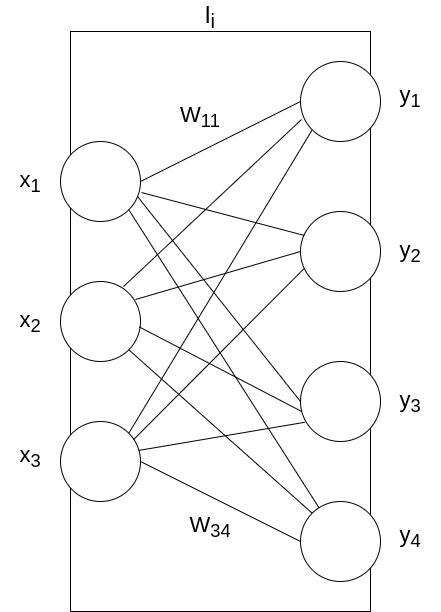
\includegraphics[width=0.3\textwidth]{../assets/linear-layer-example.png}
    \end{figure}
\end{frame}

\begin{frame}
    \frametitle{Exploding/vanishing gradients}
    
    A weight in the early layer might have a big impact on the result, thus the gradient will be very small.
    \begin{figure}
        \centering
        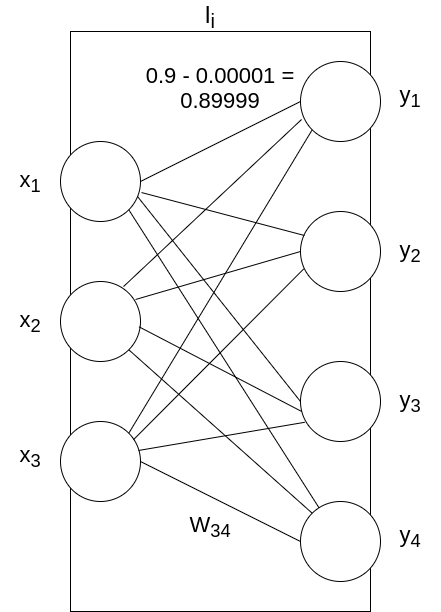
\includegraphics[width=0.3\textwidth]{../assets/linear-layer-vanishing-gradient.drawio.png}
    \end{figure}
\end{frame}

\subsection{Batch normalization layer}

\begin{frame}
    \frametitle{Batch normalization layer}

    A way to deal with the Vanishing gradients problem is by using Batch normalization layers.

    \begin{itemize}
        \item New standard deviation and mean
        \item Changes impact on final result
    \end{itemize}

    \pause
    Standardize input
    $$\hat{x} = \frac{x - E[x]}{\sqrt{Var[x]}}$$
    \pause
    Introduce new trainable parameter $\beta$ and $\gamma$
    $$y = \frac{x - E[x]}{\sqrt{Var[x]}} \cdot \gamma + \beta$$
\end{frame}

\subsection{ResNet}

\begin{frame}
    \frametitle{ResNet}

    \begin{itemize}
        \item Deeper networks seem to be more accurate
        \item Depth limit - more layers degrade accuracy
        \item ResNet can have many more layers than previous models
    \end{itemize}
\end{frame}

\begin{frame}
    \frametitle{ResNet}
    \framesubtitle{Shortcut connections}

    \begin{itemize}
        \item Skips layers
        \item Brings more accuracy
        \item Also deals with vanishing gradients problem
    \end{itemize}

    \begin{figure}
        \centering
        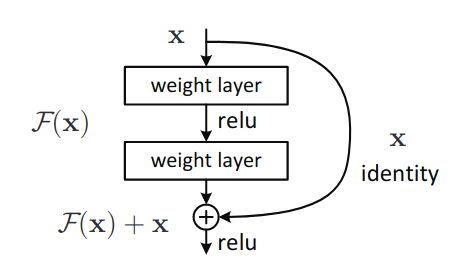
\includegraphics[width=0.55\textwidth]{../assets/shortcut-connection.png}
        \caption{A shortcut connection represented by the arching arrow. $\mathcal{F}(\bm{x})$ is the function of applying $\bm{x}$ to the two layers. $\mathcal{F}(\bm{x}) + \bm{x}$ is the value after the shortcut connection. Source: \cite{resnet}}
        \label{fig:shortcut_connection}
    \end{figure}
\end{frame}

\begin{frame}
    \frametitle{Resnet}
    \framesubtitle{Residual learning}
    
    \begin{itemize}
        \item Uses shortcut connections
        \item Cheap computational cost
        \item Good tradeoff
    \end{itemize}

    \pause

    Data before and after a shortcut connection should have the same dimensions.
    \pause

    If not the data is projected by downsampling.
\end{frame}

\begin{frame}
    \frametitle{ResNet}
    \framesubtitle{Network architectures}
    \textbf{Plain network}: $3 \times 3$ convolutions. \pause (i) layers have the same number of kernels. \pause (ii) If the feature map is halved, double the filters. \pause
    Ends with fully connected layer with 1000 outputs.

    \pause

    \textbf{Residual network}: Based on plain network, with shortcut connections. Downsampled by $1 \times 1$ convolution.
    \pause
    Batch normalization layers after each layer.
\end{frame}

\begin{frame}
    \frametitle{Resnet}
    \framesubtitle{Network architectures}
    
    Source: \cite{resnet}
    \begin{figure}
        \centering
        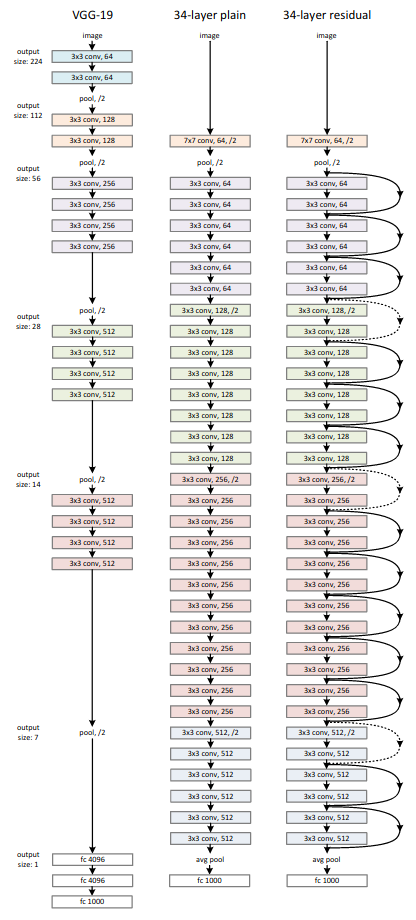
\includegraphics[scale=0.69]{../assets/residual-net.png}
        \caption{The first part of each layer tells which type of layer it is, the second tells how many channels the layer uses, and the third tells if there is downsampling ($/2$). \textbf{middle}: 34-layer plain network. \textbf{right}: 34-layer residual network - based on plain, but with shortcut connections. The dotted lines represent a downsampling in the shortcut connection. Source: \cite{resnet}}
        \label{fig:resnet}
    \end{figure}
\end{frame}

\section{Automatic differentiation}

\begin{frame}
    \frametitle{Automatic differentation}
    
    \begin{itemize}
        \item Differentiation used with network training
        \item Manually differentiating
        \item Software maintainance
    \end{itemize}
\end{frame}

\subsection{Methods of differentitation}

\begin{frame}
    \frametitle{Methods of differentiation}
    
    \begin{itemize}
        \item Manual differentiation
        \pause
        \item Numerical differentiation
    \end{itemize}

    Approximating the derivative, by finding the tangent.

    $$\frac{\partial f(\bm{x})}{\partial x_i} \approx \frac{f(\bm{x} + h\bm{e}_i) - f(\bm{x})}{h}$$

    \begin{description}
        \item[h] Very small number
        \item[$e_i$] $i$th unit vector
    \end{description}
\end{frame}

\begin{frame}
    \frametitle{Methods of differentitaion}
    \framesubtitle{Symbolic differentiation}
    
    Used by math programs (Maple).

    Works by systematically applying rules.
\end{frame}

\subsection{Automatic differentitaion}

\begin{frame}
    \frametitle{Automatic differentiation}
    
    \begin{itemize}
        \item When we do not need the symbolic form ($f(x) = \sin (x) \cdot 2$)
        \item Returns numeric values
        \item Significantly simplify
        \item Branching and loops
    \end{itemize}
\end{frame}

\subsection{Forward mode}

\begin{frame}[fragile]
    \frametitle{Automatic differentiation}
    \framesubtitle{Forward mode}
    
    Conceptually the most simple mode.
    \pause

    Consider a function $F(x, y) = \sin (x) + x \cdot y$
    \pause
    
    Storing each intermediate value as
    \begin{lstlisting}[label={lst:autodiff_fwd_trace}, caption={Forward trace of a simple function $f(x, y) = \sin(x) + x\cdot y$}]
w-1 = y
w0 = x
w1 = sin(w0)
w2 = w0 * w-1
w3 = w1 + w2
r = w3
    \end{lstlisting}
    Goal: Find the gradient
    $$\nabla F = \left[ \frac{\partial r}{\partial x}, \frac{\partial r}{\partial y} \right]$$
\end{frame}

\begin{frame}[fragile]
    \frametitle{Automatic differentation}
    \framesubtitle{Forward mode}
    
    We can expand the expression $\frac{\partial r}{\partial x}$ by applying the chain rule

    $$\frac{\partial r}{\partial x} = \frac{\partial r}{\partial w_2} \left(\frac{\partial w_2}{\partial w_1} \left(\frac{\partial w_1}{\partial x}\right) \right)$$.

    The derivative of each intermediate value can be solved by using the chain rule.

    \begin{lstlisting}[label={lst:autodiff_fwd_deriv}]
w-1' = 1
w0' = 1
w1' = cos(w0) * w0'
w2' = w-1'
w3' = w1' + w2'
r' = w3'
    \end{lstlisting}
    \pause
    To obtain the gradient, we do this process for each input parameter
\end{frame}

\subsection{Reverse mode}

\begin{frame}
    \frametitle{Automatic differentiation}
    \framesubtitle{Reverse mode}
    
    \begin{itemize}
        \item Forward mode has to find the derivative for each input
        \item Costly for neural networks
        \item Reverse mode derives once for each output.
    \end{itemize}

    \pause

    Works by finding the adjoint for each intermediate variable $w_i$.
    $$\bar{w_i} = \frac{\partial y_j}{\partial w_i}$$

\end{frame}

\begin{frame}[fragile]
    \frametitle{Reverse mode}
    
    Values are recorded during inital forward trace.

    The adjoint represents how sensitive output $y_j$ is to the changes in the intermediate variable $w_i$.

    \pause

    Forward trace
    \begin{lstlisting}[basicstyle=\tiny]
w-1 = y
w0 = x
w1 = sin(w0)
w2 = w0 * w-1
w3 = w1 + w2
r = w3
    \end{lstlisting}

    Reverse trace
    \begin{lstlisting}[basicstyle=\tiny, label={lst:autodiff_rev_trace}]
_y   = _w-1                                       = 5
_x   = _w0                                        = 1.58
_w0  = _w0 + _w1 d w1 / d w0  = _w0 + 1 * cos(w0) = 2 - 0.42 = 1.58
_w-1 = _w2 d w2 / d w-1       = _w2 * (w0)        = 1 * 5 = 5
_w0  = _w2 d w2 / d w0        = _w2 * (w-1)       = 1 * 2 = 2
_w2  = _w3 d w3 / d w2        = _w3 * 1           = 1
_w1  = _w3 d w3 / d w1        = _w3 * 1           = 1
_w3  = d r / d r              = 1
    \end{lstlisting}
    \pause

    $$\nabla F = \left( \begin{array}{c}
        \bar{x}\\
        \bar{y}
    \end{array} \right) = \left( \begin{array}{c}
        1.58\\
        5
    \end{array} \right)$$
\end{frame}

\section{Optimizing matrix multiplication}

\begin{frame}
    \frametitle{Optimizing matrix multiplication}
    
    \begin{itemize}
        \item Common mathematical function
        \item Fully connected and convolutional layers could benefit
        \item Not implemented in this project
        \item Highly parallel
        \item Effecient algorithms are not trivial
        \item Memory reuses $O(n)$
    \end{itemize}
\end{frame}

\begin{frame}
    \frametitle{Effecient matrix multiplication}
    
    \begin{itemize}
        \item Use blocks that fit into shared memory
        \item Utilize caching and coalesced access
    \end{itemize}

    \begin{figure}
        \centering
        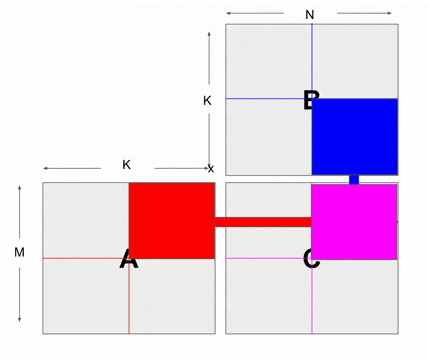
\includegraphics[width=0.35\textwidth]{../assets/gemm.png}
        \caption{A visual representation of how to tiles in $A$ and $B$ might be added together in $C$. Source: \cite{gemm}}
        \label{fig:gemm}
    \end{figure}

    To utilize even more parallelism, store each addition to $C$ in an array for that entry, then sum later.
\end{frame}

\section{Design and implementation}

\begin{frame}
    \frametitle{Design}
    
    \begin{itemize}
        \item Created using Futhark
        \item Limitations
        \item \texttt{fold}-like idea
    \end{itemize}

    Repository can be found at \texttt{github.com/Alexnortung/futhark-nn}
\end{frame}

\subsection{Layers}

\begin{frame}[fragile]
    \frametitle{Design}
    \framesubtitle{Layers}
    
    \begin{itemize}
        \item Each layer has it's own module
        \item Combining layers
        \item Layer options (stride, padding, etc.)
        \pause
        \item Weights as single argument
    \end{itemize}

    \begin{lstlisting}
val vjp 'a 'b : (f: a -> b) -> (x: a) -> (y': b) -> a
    \end{lstlisting}

    \pause

    \begin{lstlisting}[basicstyle=\tiny]
type^ layer_fwd_type 'options 'layer_input 'wb 'out = (k: i64) -> options -> [k]layer_input -> wb -> [k]out
type^ layer_apply_optimize_type 't 'options 'weights = options -> optimizer_apply_record t -> weights -> weights -> weights
type^ layer_type 't 'options 'layer_input 'wb 'shape 'out = {
    forward: layer_fwd_type options layer_input wb out,
    apply_optimize: layer_apply_optimize_type t options wb,
    options: options,
    weights: wb,
    shape: shape
}
    \end{lstlisting}
\end{frame}

\begin{frame}[fragile]
    \frametitle{Neural network}
    
    The neural network type is expressed as

    \begin{lstlisting}[basicstyle=\tiny]
type^ nn_type 't 'shape_type 'input 'output 'current_weight 'rest_weights = {
    seed: i32,
    shape: shape_type,
    forward:(k: i64) -> [k]input -> (current_weight, rest_weights) -> [k]output,
    apply_optimize: (optimizer_apply_record t) -> (current_weight, rest_weights) -> (current_weight, rest_weights) -> (current_weight, rest_weights),
    weights: (current_weight, rest_weights)
}
    \end{lstlisting}

    \begin{itemize}
        \item Combination of weights
        \item Forward propagation with weights as last parameter
    \end{itemize}
\end{frame}

\begin{frame}[fragile]
    \frametitle{Combining layers}
    
    \begin{lstlisting}[basicstyle=\tiny]
def add_layer 'nn_input 'l_input 'l_options  'l_wb 'l_shape 'l_out 'nn_shape 'prev_current_weight 'prev_rest_weight
(layer: layer_type t l_options l_input l_wb l_shape l_out)
(network:nn_type nn_shape nn_input l_input prev_current_weight prev_rest_weight)
: nn_type l_shape nn_input l_out l_wb (prev_current_weight, prev_rest_weight) =
    let {
        apply_optimize = layer_apply_optimize,
        forward = layer_forward,
        options = layer_options,
        weights = layer_weights,
        shape = layer_shape
    } = layer
    let { shape = _, apply_optimize, weights, forward, seed } = network
    let new_forward = (\k -> compose_forward (forward k) (layer_forward k layer_options))
    let new_apply_optimize = compose_apply_optimize apply_optimize (layer_apply_optimize layer_options)
    in {
        seed,
        shape = layer_shape,
        weights = (layer_weights, weights),
        apply_optimize = new_apply_optimize,
        forward = new_forward
    }
    \end{lstlisting}
\end{frame}

% \begin{frame}[fragile]
%     \frametitle{Initializing the network}
%     
% \end{frame}

\begin{frame}[fragile]
    \frametitle{Interface}
    
    \begin{itemize}
        \item Time consuming
        \item Abstract away implementation details
        \item input/output sizes
        \item Making it as safe as possible
    \end{itemize}

    The \texttt{add\_layer} is the general function, we can make shorthand functions to add layers of different types of layers to the network.
    \begin{lstlisting}
def linear 'rest_weights 'input_type 'prev_current_weight 'prev_rest_weight [m]
    (n: i64)
    (activation: activation_type t)
    (network: nn_type shape_1d input_type ([m]t) prev_current_weight prev_rest_weight)
    \end{lstlisting}
\end{frame}

\begin{frame}[fragile]
    \frametitle{Interface}
    \framesubtitle{Example}
    
    \begin{itemize}
        \item Convolutional and maxpool needs output sizes
        \item \texttt{|>} convenience
    \end{itemize}
    \begin{lstlisting}[basicstyle=\tiny]
let net = nn.init_3d 1 28 28 seed
|> nn.conv_2d 26 26 32 3 3 (nn.activation.relu)
|> nn.conv_2d 24 24 64 3 3 (nn.activation.relu)
|> nn.add_layer (nn.layers.dimension.from_3d_2d 24 (24 * 64))
|> nn.maxpool_2d 12 (12 * 64) -- window size 2 2
|> nn.add_layer (nn.layers.dimension.from_2d_1d (12 * 12 * 64))
|> nn.linear 128 (nn.activation.relu)
|> nn.linear 10 (nn.activation.log_softmax)
    \end{lstlisting}
\end{frame}

\begin{frame}[fragile]
    \frametitle{Training the network}
    
    \begin{itemize}
        \item Loss functions
        \item Optimizers - it's own type
        \item Training
    \end{itemize}

    \begin{lstlisting}
let loss = nn.make_loss (nn.loss.mse false) net
let optimizer = nn.optim.sgd.init 0.01 (loss)
let net = nn.train input labels 50 optimizer net
    \end{lstlisting}
\end{frame}

% \begin{frame}[fragile]
%     \frametitle{Design considerations}
%     
%     \begin{itemize}
%         \item One dimensional array and shape
%     \end{itemize}
% \end{frame}

\begin{frame}[fragile]
    \frametitle{Improving the fully connected layer}
    
    The fully connected layer might be improved by using matrix multiplication

    $$\bm{Y} = \bm{\sigma} \left( \bm{B} + \bm{W} \bm{X} \right)$$
\end{frame}

\begin{frame}[fragile]
    \frametitle{Improving convolutional layer}
    
    The convolutional layer might also be improved by transforming the slices and the kernel to a matrices.

    \begin{figure}
        \centering
        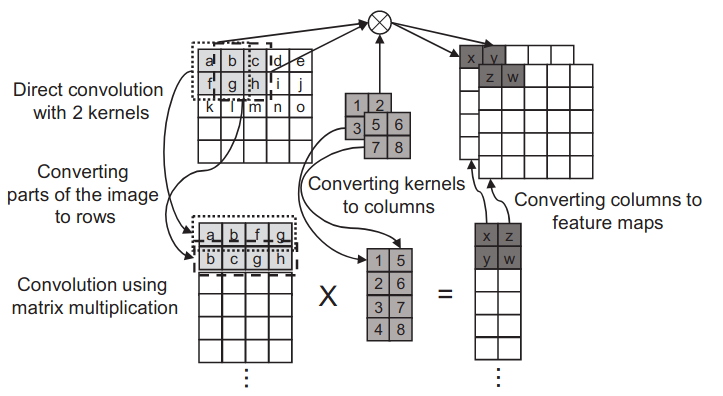
\includegraphics[width=0.8\textwidth]{../assets/conv-matrix.png}
        \caption{Direct convolution is shown in the top. The transformed data and kernel for using matrix multiplication is shown in the bottom, and the arrows shows how they aretransformed. Source: \cite{perfomance_analysis_cnn}}
        \label{fig:conv_matrix}
    \end{figure}
\end{frame}

\section{Tests}

\begin{frame}
    \frametitle{Tests}

    \begin{itemize}
        \item Unit tests for all layers and neural network
        \item Script for gathering and formatting MNIST handwritten numbers
        \item Cuda issues
        \item Attempted to benchmark with the MNIST dataset - memory issues
    \end{itemize}
\end{frame}

\section{Future work and conclusion}

\subsection{Future work}

\begin{frame}
    \frametitle{Future work}

    \begin{itemize}
        \item Optimizations
        \item Cleaning up
        \item In future versions of Futhark, make a better interface.
        \item ResNet and Batch normalization layers
    \end{itemize}
\end{frame}

\subsection{Conclusion}

\begin{frame}
    \frametitle{Conclusion}
    
    \begin{itemize}
        \item Neural networks
        \begin{itemize}
            \item Layers
            \item activation functions
            \item Loss functions
            \item ResNet
        \end{itemize}
        \item Automatic differentiation
        \item Optimizing Matrix multiplication
        \item Implementation
        \item Tests
    \end{itemize}
\end{frame}

\begin{frame}
    \frametitle{References}
    
    % \printbibliography
\end{frame}

\end{document}
